
\documentclass[11pt]{exam} % https://www.ctan.org/pkg/exam?lang=en

\usepackage[lmargin=1.in,rmargin=1.in,tmargin=1.in,bmargin=1in]{geometry}
\usepackage{setspace}
\usepackage[pdftex]{graphicx}
\usepackage{titling}
\usepackage[
	pdfauthor={Brian Weinstein},
	pdftitle={Homework 1},
	bookmarks=true,
	colorlinks=true,
	linkcolor=blue,
	urlcolor=blue,
	citecolor=blue,
	pdftex,
	linktocpage=true
	]{hyperref}
\usepackage[textsize=tiny]{todonotes}
\usepackage{float}
\setlength\parindent{0pt}
\usepackage{lipsum}
\usepackage{amsmath}


\qformat{\textbf{Problem \thequestion: \thequestiontitle}\quad \hfill}


\pagestyle{headandfoot}
\runningheadrule
\firstpageheader{}{}{}
\runningheader{\theauthor}{\thetitle}{\thedate}
\firstpagefooter{}{\thepage}{}
\runningfooter{}{\thepage}{}


\usepackage{xcolor}
\usepackage{adjustbox}
\usepackage{verbatim}
\definecolor{shadecolor}{rgb}{.9, .9, .9}

\newenvironment{code}%
   {\par\noindent\adjustbox{margin=1ex,bgcolor=shadecolor,margin=0ex \medskipamount}\bgroup\minipage\linewidth\verbatim}%
   {\endverbatim\endminipage\egroup}

\newenvironment{codeSmall}%
   {\par\noindent\adjustbox{margin=1ex,bgcolor=shadecolor,margin=0ex \medskipamount}\bgroup\minipage\linewidth\verbatim\footnotesize}%
   {\endverbatim\endminipage\egroup}

\newcommand{\ramsey}{\href{http://www.statisticalsleuth.com/}{Ramsey }}



\begin{document}


\title{STAT W4201 001, Homework 3}
\author{Brian Weinstein (bmw2148)}
\date{Feb 17, 2016}
\maketitle

Code is attached here and also posted at \href{https://github.com/BrianWeinstein/advanced-data-analysis}{https://github.com/BrianWeinstein/advanced-data-analysis}. Where relevant, code snippets and output are are included in-line.

\begin{questions}


\titledquestion{\ramsey 4.30} % Problem 1
\todo{Problem 1: done, but maybe shouldn't be using the t test?}

A boxplot of SPF estimates for each subject is shown in Figure \ref{fig:1}, where the SPF estimate is calculated for each subject as the number minutes that a person was able to withstand sunlight before applying sunscreen divided by the number of minutes they were able to withstand after applying sunscreen. The dataset contains paired observations, and the quantity in question has a nearly normal distribution with no outliers, making it a strong candidate for the one-sample paired t-test.

\begin{codeSmall}
   PreTreatment Sunscreen spfEstimate
1            30       120    4.000000
2            45       240    5.333333
3           180       480    2.666667
4            15       150   10.000000
5           200       480    2.400000
6            20       270   13.500000
7            15       300   20.000000
8            10       180   18.000000
9            20       300   15.000000
10           20       240   12.000000
11           60       480    8.000000
12           60       300    5.000000
13          120       480    4.000000
\end{codeSmall}

\begin{figure}[!h]
	\centering
	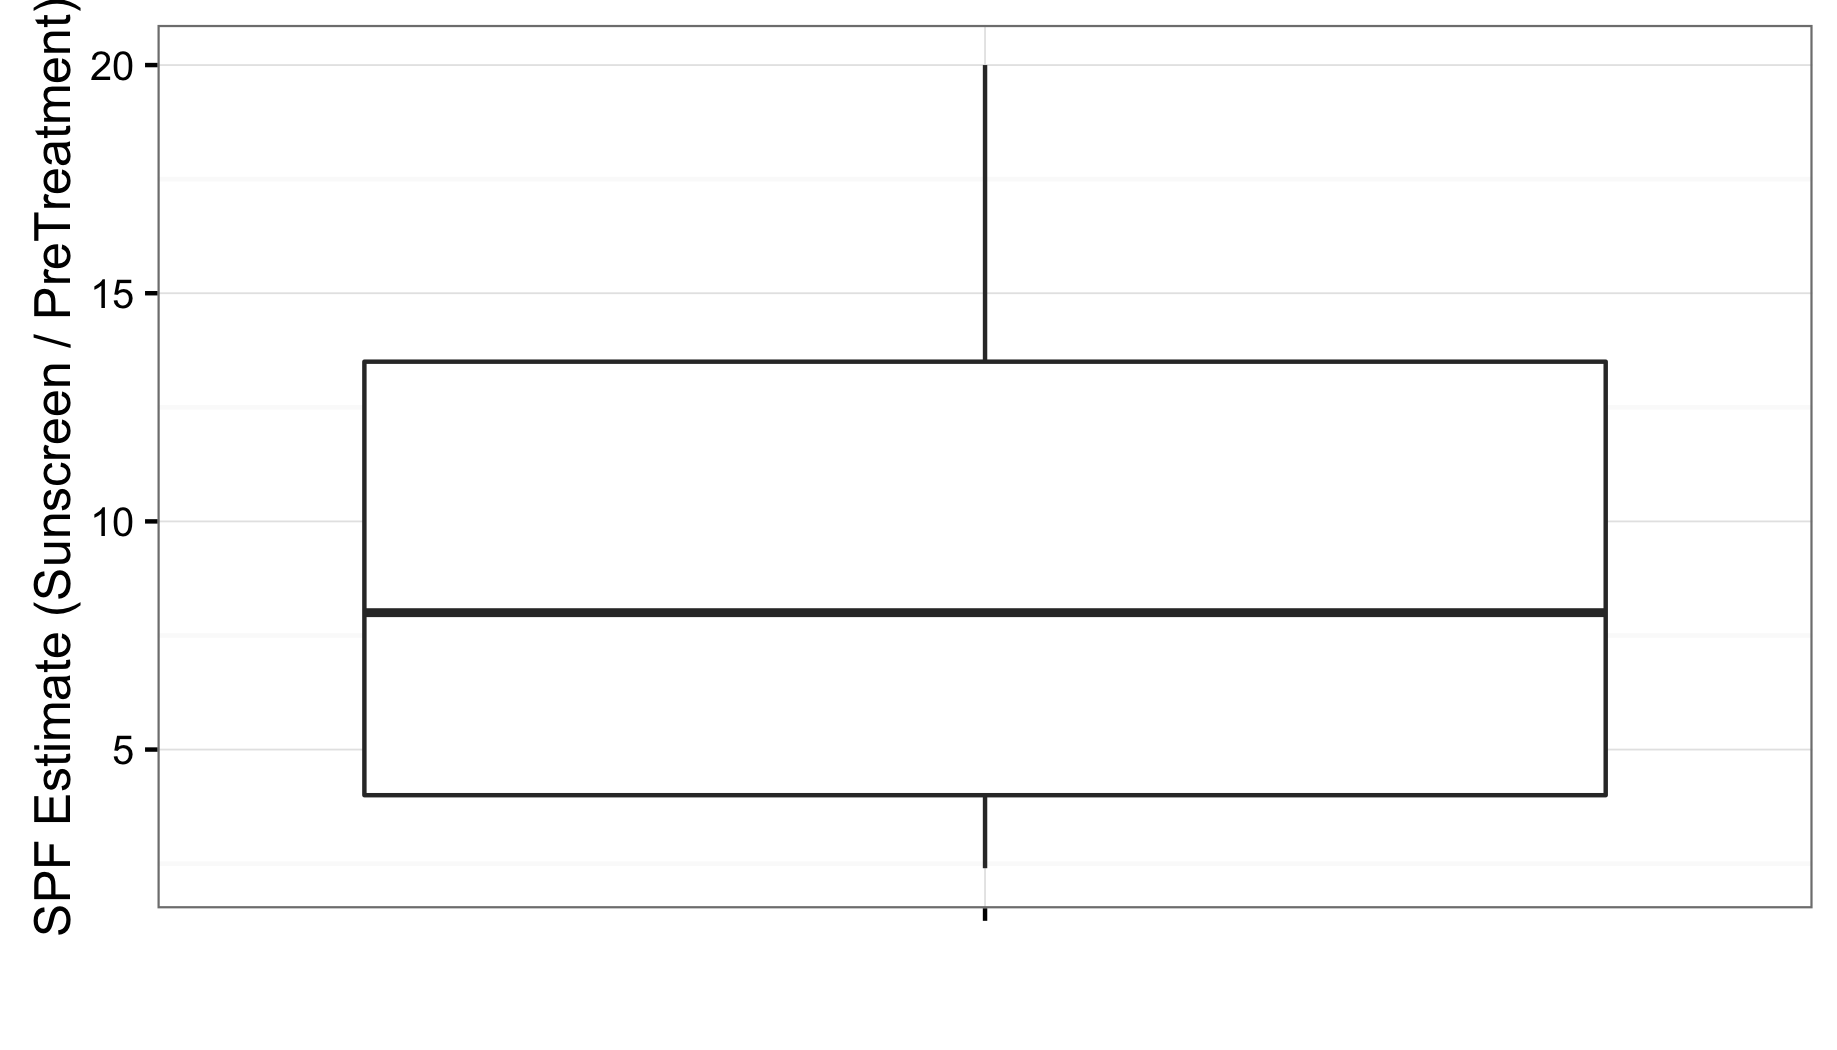
\includegraphics[width=4.25in]{1.png}
	\caption{SPF estimates for 13 subjects.}
	\label{fig:1}
\end{figure}

The SPF Estimate has a mean of of $9.223$, and the standard error on the mean is $\text{SD}(spfEstimate)/\sqrt{13} = 1.664$. Using a t distribution with $(13-1)=12$ degrees of freedom, a 95\% confidence interval for the mean is

\begin{gather*}
9.223 \pm t_{12}(1-(0.05/2) \times 1.664 \\
9.223 \pm (2.179)(1.664) \\
9.223 \pm 3.626 \\
\Rightarrow \text{95\% CI for the mean SPF Estimate: } [5.598, 12.848]
\end{gather*}


A potentially confounding variable could be the strength of sunlight during the measurement period for each subjects' data points. For a given participant, if the sunlight strength wasn't constant for both measurements, it likely would have had an impact on the duration for which they were able to withstand the sunlight.


\titledquestion{\ramsey 4.32} % Problem 2
\todo{Problem 2: done}

See attached code. A boxplot of the difference in the number of retching episodes while on the marijuana treatment vs the placebo is show in Figure \ref{fig:2}.

The data provides convincing evidence that marijuana reduced the frequency of retching episodes compared to the placebo (estimated one-sided p-value = $0.000156$ from the sign test). The marijuana treatment reduced the number of retching episodes for a given patient by an estimated 25 episodes (95\% confidence interval for an additive treatment effect: 7 to 43 episodes).

\begin{figure}[!h]
	\centering
	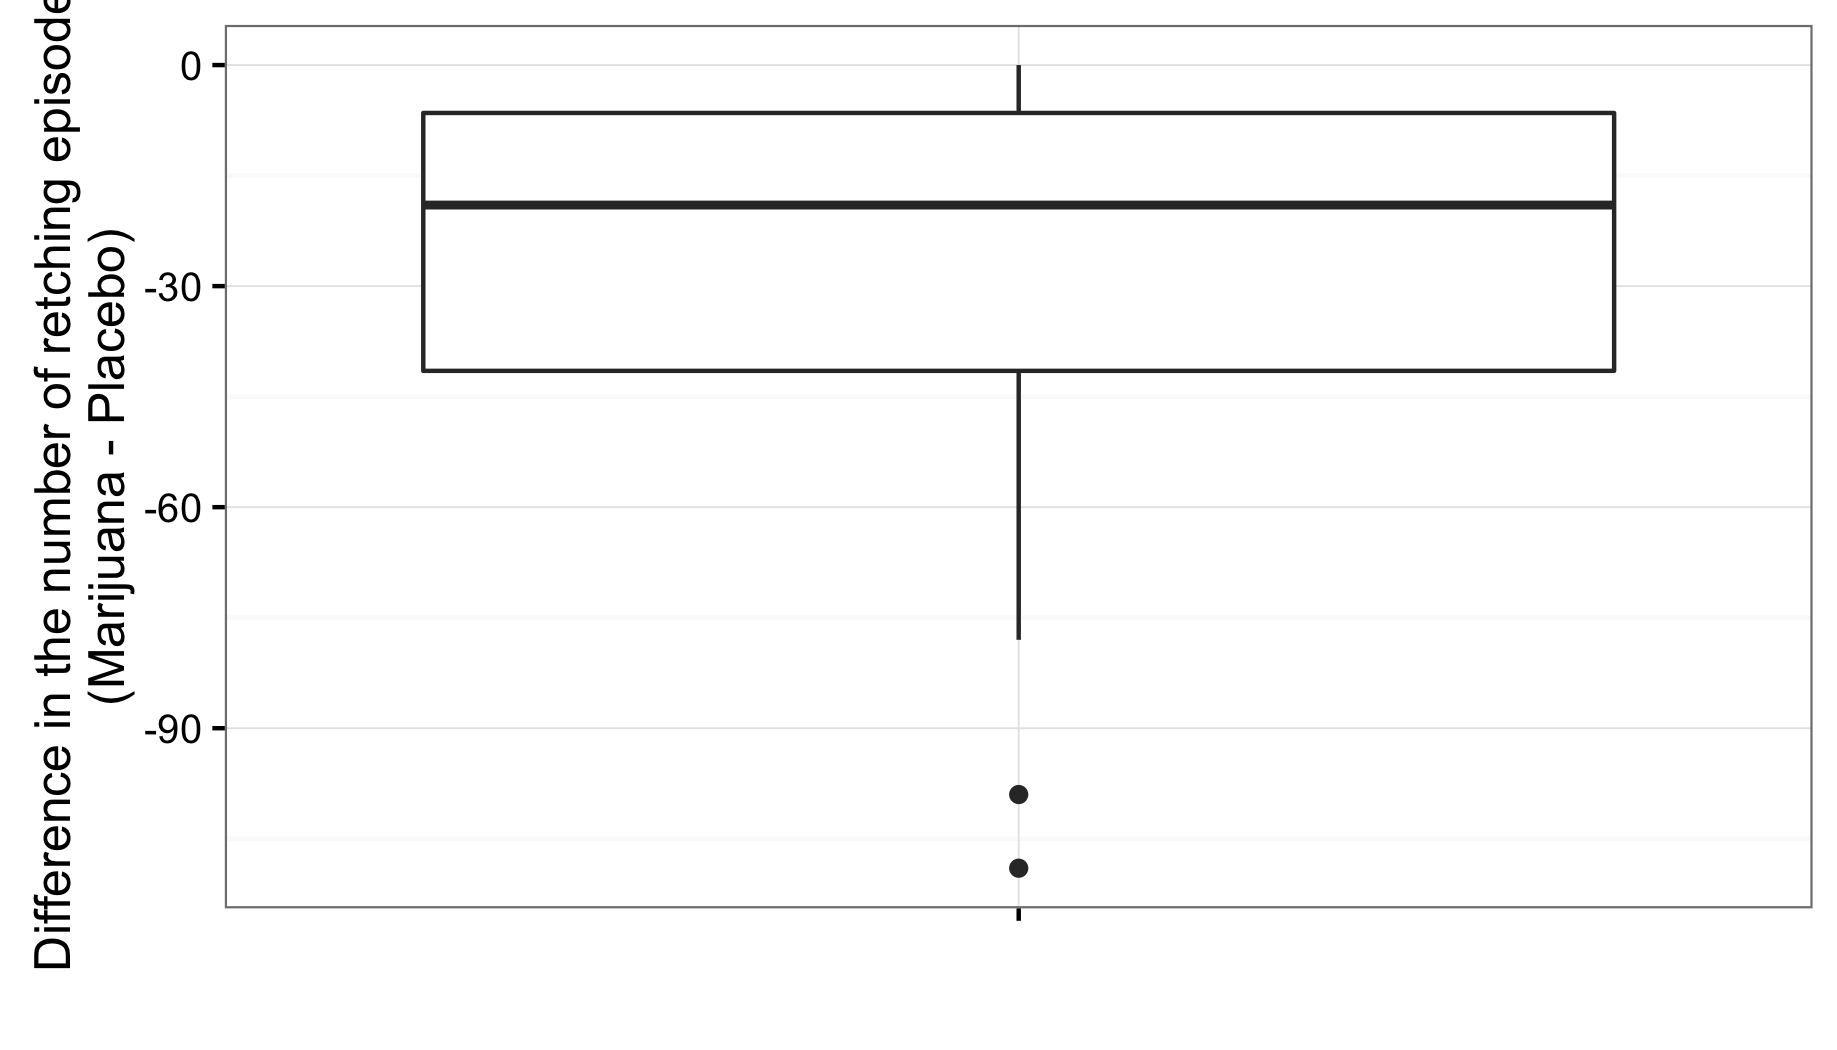
\includegraphics[width=4.25in]{2.png}
	\caption{The difference in the number of retching episodes for 15 patients while on a marijuana treatment vs a placebo.}
	\label{fig:2}
\end{figure}





\titledquestion{\ramsey 5.19} % Problem 3
\todo{Problem 3: errors}


\begin{parts}

\part The pooled estimate of the variance $s_p^2$ is given by

\begin{equation*}
\begin{split}
s_p^2 &= \frac{\sum_{i=1}^{I} (n_i -1 ) s_i^2}{\sum_{i=1}^{I} (n_i -1 )} \\
&= \frac{   (127-1)(0.4979)^2  +  (44-1)(0.4235)^2  +  (24-1)(0.3955)^2  +  \cdots  }{(127-1) +  (44-1) +  (24-1)  +  \cdots} \\
& \quad \quad \quad \frac{\cdots + (41-1)(0.3183)^2 + (18-1)(0.3111)^2  +  (16-1)(0.4649)^2 + \cdots}{\cdots + (41-1) + (18-1)  +  (16-1) + \cdots } \\
& \quad \quad \quad \frac{\cdots  +  (11-1)(0.2963)^2  +  (7-1)(0.3242)^2  +  (6-1)(0.5842)^2  }{\cdots +  (11-1) +  (7-1)  +  (6-1)} \\
&= 0.1919.
\end{split}
\end{equation*}

\part To construct an ANOVA table to test for species differences, we first compute $SS_W$, the sum of squared residuals of the ``within'' group.

\begin{align*}
SS_W &= \sum_{i=1}^9 \left[ \sum_{j=1}^{n_i} \left( Y_{ij} - \overline{Y_i} \right)^2  \right] = \sum_{i=1}^9 \left[ (n_i - 1) \text{SE}(Y_i)  \right] \\
&= (127 - 1)(0.4979) + (44 - 1)(0.4235) + \cdots + (6 - 1)(0.5842) \\
&= 122.8658.
\end{align*}

Given the sample standard deviation of all 294 observations as one group is $\text{SD}_{Total} = 0.4962$, the total sum of squared residuals $SS_{Total}$ is

\todo{\quad Should SS total be -9 (-I) instead of -1 ?}
\begin{align*}
SS_{Total} &= \sum_{i=1}^9 \left[ \sum_{j=1}^{n_i} \left( Y_{ij} - \overline{Y} \right)^2  \right] = (n_1 + n_2 + \cdots + n_9 - 1) (\text{SD}_{Total}) \\
&= (127 + 44 + \cdots + 6 - 1)(0.4962) =  (293)(0.4962)\\
&= 145.3866.
\end{align*}

Therefore, the sum of squared residuals of the ``between'' group, $SS_B$ is:
$$SS_B = SS_{Total} - SS_W = 145.3866 - 122.8658 = 22.5208.$$

The Total, Within, and Between degrees of freedom are $\text{df}_{Total} = (n-1) = 293$, $\text{df}_W = (n-I)=(294-9) = 285$, and $\text{df}_B = \text{df}_{Total} - \text{df}_W  = 8$, respectively. \\

The Mean Square for the Within and Between groups is the [(Sum of Squares) / df], and the F-statistic is defined as the [(Between Mean Square) / (Within Mean Square)]. \\

Thus the ANOVA table to test for species differences is:

\begin{center}
  \begin{tabular}{ l c c c c c}
    Source of Variation & Sum of Squares & d.f. & Mean Square & F-Statistic & p-Value \\ \hline \hline
    Between Groups & 22.5208 & 8 & 2.8151 & 6.5300 & $8.0551 \times 10^{-8}$ \\
    Within Groups & 122.8658 & 285 & 0.4311 & & \\ \hline
    Total & 145.3866 & 293 & & &
  \end{tabular}
\end{center}

\quad \linebreak
Where the p-value for the F-Statistic is given by the CDF of an F distribution with 8 and 285 degrees of freedom.
\begin{codeSmall}
> # p-value of F-statistic
> pf(q=6.5300, df1=8, df2=285, lower.tail=FALSE)
[1] 8.055137e-08
\end{codeSmall}



\part The ANOVA method for calculating $SS_B$ yields the same answer as the formula:

$$ SS_B = \sum_{i=1}^I \left( n_i \overline{Y_i}^2 \right) - n\overline{Y}^2 = \sum_{i=1}^9 \left( n_i \overline{Y_i}^2 \right) - n\overline{Y}^2 .$$

The overall mean $\overline{Y}=7.4746$ is computed as a weighted average of the group means and $n=294$, thus \todo{\quad 17.45402 != 22.5208 : maybe my SS total calc is incorrect?}
\begin{align*}
SS_B &= \sum_{i=1}^9 \left( n_i \overline{Y_i}^2 \right) - n\overline{Y}^2 \\
&= (127)(7.347)^2 + (44)(7.368)^2 + (24)(7.418)^2 + (41)(7.487)^2 + (18)(7.563)^2 + \cdots \\
& \quad \quad \quad \cdots + (16)(7.568)^2 + (11)(8.214)^2 + (7)(8.272)^2 + (6)(8.297)^2 - (294)(7.4746)^2 \\
&= 17.45402
\end{align*}


\part If the first 6 species have one common mean and the last 3 have another common mean, we find that \todo{\quad finish 3d}




\end{parts}







\titledquestion{} % Problem 4
\textit{Consider the Bumpus's data in Chapter 2, compute the power of the two-sided two sample t-test of size 0.05 (i.e., reject the null hypothesis if the absolute value the t-statistic is greater than or equal to 2), under the alternative that $\mu_x - \mu_y = \overline{x} - \overline{y} = 0.01$ and $\sigma = s_p = 0.0214$.}
\todo{Problem 4: not started}



\titledquestion{} % Problem 5
\textit{Show that the two-sided two sample t-test is equivalent to the anova F-test, if the number of groups is two.}
\todo{Problem 5: incomplete}


For $I=2$ groups, the F-statistic is given by
$$ \text{F-statistic} =  \frac{SS_B / \left[ (n-1) - (n-I) \right]}{SS_W / (n-I)}, $$
where $n_1$ and $n_2$ are the sizes of samples 1 and 2, respectively, $n=n_1+n_2$ is the total sample size, $SS_B$ is the ``between groups'' sum of squared residuals, and $SS_W$ is the ``within groups'' sum of squared residuals.

Simplifying, we find
$$\text{F-statistic} =  \frac{SS_B / (I-1) }{SS_W / (n-I)} = \frac{SS_B / (2-1) }{SS_W / (n-2)} = \frac{SS_B / 1 }{SS_W / (n-2)}.$$

If the observations from group 1 are $\sim \text{N}(\mu_1, \sigma^2)$ and the observations from group 2 are $\sim \text{N}(\mu_2, \sigma^2)$, we know that
$$\text{F-statistic} \sim \text{F}_{1, n-2} \text{ , which is equivalent to }t^2_{n-2}.$$
i.e., an F distribution with a numerator degrees of freedom of 1 and a denominator degrees of freedom of $n-2$ is equivalent to the square of a t distribution with $n-2$ degrees of freedom.



\titledquestion{} % Problem 6
\textit{Consider $X_1,\ldots,X_{10}$ are i.i.d. N($0,\sigma^2$), $Y_1,\ldots,Y_{10}$ are i.i.d. N($\mu,\sigma^2$) and hypothesis testing:}
\begin{align*}
H_0 &: \mu = 0\\
H_A &: \mu \neq 0.
\end{align*}
\textit{Compute the power of a two sided two sample t-test of size 0.05 when $\sigma^2 = 1$ and $\mu =$ 0.1, 0.5, 1, and 2. Plot the power as a function of $\mu$. Then, increase the sample size in each group to 20 and draw the power function in the same plot as that of the sample size 10.}
\todo{Problem 6: done}

See attached code. A plot of the power for a two-sided, two-sample t-test of size 0.05, for $\sigma^2 =1$, $\mu = \{0.1, 0.5, 1, 2 \}$, and $(n_1, n_2) = \{(10,10), (20,20)\}$ is shown in Figure \ref{fig:6}.

\begin{figure}[!h]
	\centering
	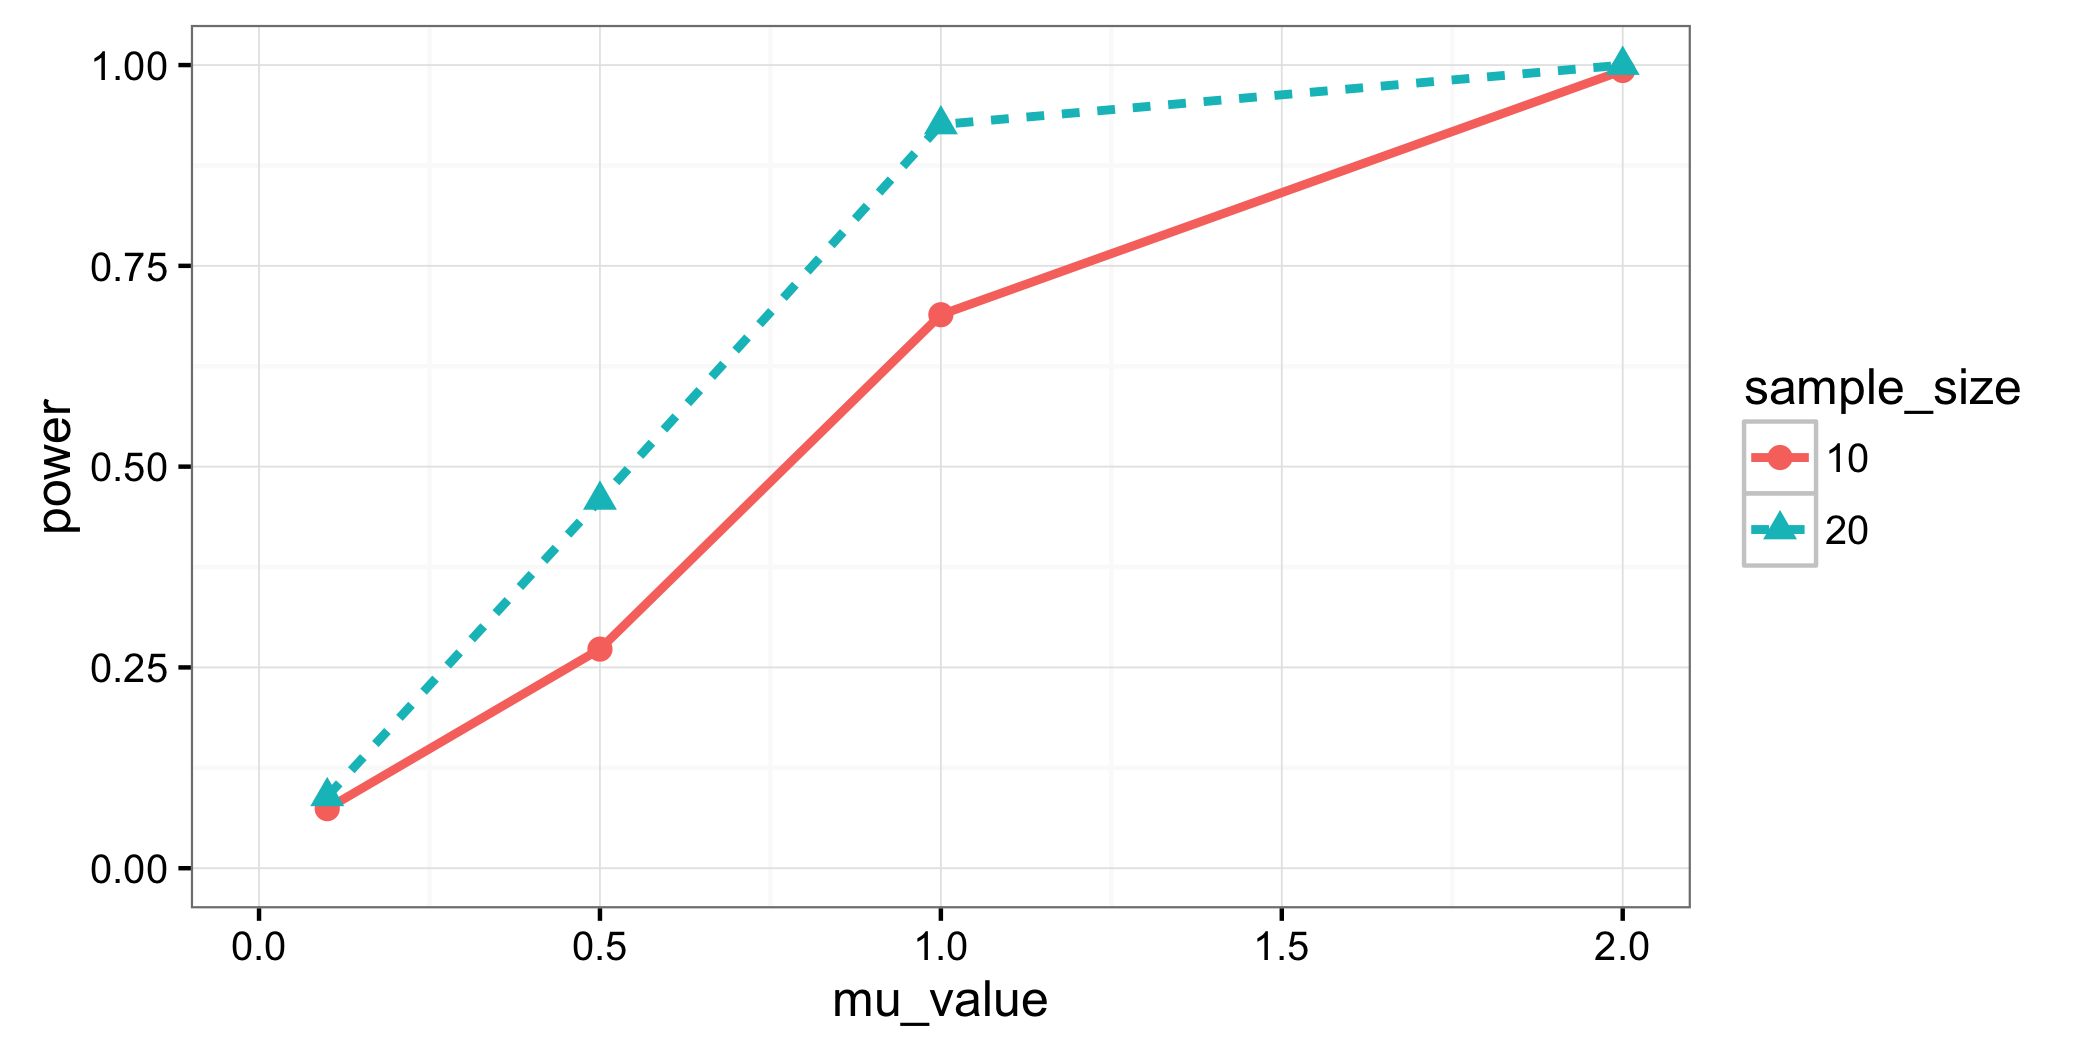
\includegraphics[width=4.25in]{6.png}
	\caption{The power of a two-sided, two-sample t-test of size 0.05 at various sample sizes and $\mu$ values.}
	\label{fig:6}
\end{figure}



\titledquestion{} % Problem 7
\textit{Under the setting of the previous problem, show that, under the null hypothesis, the p-value follows the uniform distribution on the interval [0, 1] and perform simulations to confirm it.}
\todo{Problem 7: not started}




\end{questions}

\listoftodos

\end{document}